\section{The conquers II}

\begin{figure}[htbp]
\begin{center}
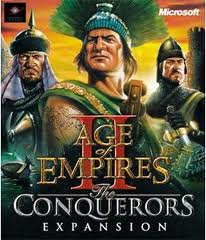
\includegraphics[width=.37\textwidth]{./imagenes/conquers.jpg}
\caption{The conquers II}
\label{The conquers II}
\end{center}
\end{figure}
The conquers II  es un videojuego de estrategia en tiempo real para computadoras personales, desarrollado por Ensemble Studios y publicado por Microsoft Games para las plataformas Microsoft Windows y Apple Macintosh. El título expande al videojuego Age of Empires II: The Age of Kings y fue lanzado a mediados del año 2000.
Mantiene el mismo guion en su desarrollo tanto económico como militar, no obstante introduce algunas mejoras en la IA de algunas unidades que ayudan a tener más tiempo para plantear una estrategia, introduciendo civilizaciones americanas (Mayas y Aztecas), además de algunas otras civilizaciones (Españoles, Hunos y Coreanos), más modos de juego y nuevos mapas.

\subsubsection{¿Por qué es uno de mis juegos favoritos?}
\begin{itemize}
\item[Keyla Figueroa] Este juego se basa en armar estrategias, tanto de ataques como de defensa. 
El juego comienza con cierta cantidad de aldeanos, a estos se les asigna diferentes tareas como recolectar madera, alimentos, oro y roca. En base a lo que ellos recolectan, se construyen casas, establos, cuarteles, etc, hasta llegar a armar un imperio con tus propias reglas. El objetivo principal de este juego es derrotar a todos los imperios existentes, quedando así como el único imperio conquistador.
Lo que más me gusta de este juego es que estimula el cerebro al momento de tomar decisiones, a liderar frente a diversas situaciones, y a conocer más sobre las culturas occidentales y orientales del mundo. 
\end{itemize}